% SPDX-FileCopyrightText: 2026 Cyprien PIERRE
% SPDX-License-Identifier: CC-BY-4.0
\documentclass[tikz,border=5pt]{standalone}
\usepackage[T1]{fontenc}
\usepackage{lmodern}
\usetikzlibrary{arrows.meta,positioning}
\begin{document}
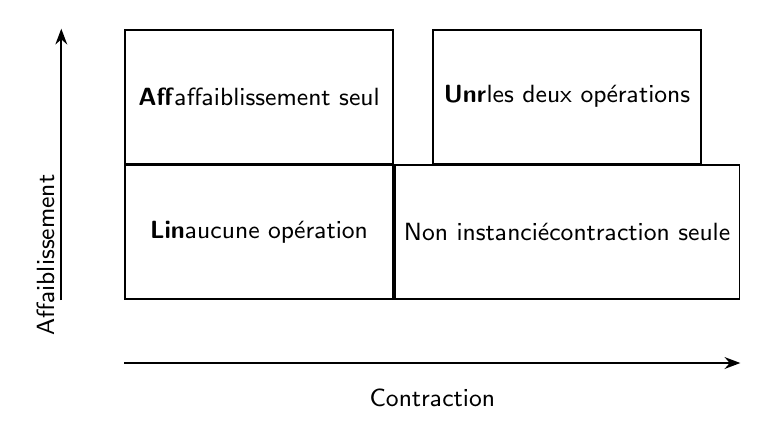
\begin{tikzpicture}[
  font=\sffamily\small,
  cell/.style={draw, minimum width=34mm, minimum height=17mm, align=center, line width=.65pt},
  axis/.style={-{Stealth[length=2mm]}, line width=.75pt}
]
\node[cell] (lin) at (0,0) {\textbf{Lin}\par aucune opération};
\node[cell, right=0pt of lin] (relevant) {Non instancié\par contraction seule};
\node[cell, above=0pt of lin] (aff) {\textbf{Aff}\par affaiblissement seul};
\node[cell, above=0pt of relevant] (unr) {\textbf{Unr}\par les deux opérations};
\draw[axis] ([yshift=-8mm]lin.south west) -- ([yshift=-8mm]relevant.south east)
  node[midway, below=2mm] {Contraction};
\draw[axis] ([xshift=-8mm]lin.south west) -- ([xshift=-8mm]aff.north west)
  node[midway, left=2mm, rotate=90] {Affaiblissement};
\end{tikzpicture}
\end{document}